
%% bare_jrnl.tex
%% V1.3
%% 2007/01/11
%% by Michael Shell
%% see http://www.michaelshell.org/
%% for current contact information.
%%
%% This is a skeleton file demonstrating the use of IEEEtran.cls
%% (requires IEEEtran.cls version 1.7 or later) with an IEEE journal paper.
%%
%% Support sites:
%% http://www.michaelshell.org/tex/ieeetran/
%% http://www.ctan.org/tex-archive/macros/latex/contrib/IEEEtran/
%% and
%% http://www.ieee.org/



% *** Authors should verify (and, if needed, correct) their LaTeX system  ***
% *** with the testflow diagnostic prior to trusting their LaTeX platform ***
% *** with production work. IEEE's font choices can trigger bugs that do  ***
% *** not appear when using other class files.                            ***
% The testflow support page is at:
% http://www.michaelshell.org/tex/testflow/


%%*************************************************************************
%% Legal Notice:
%% This code is offered as-is without any warranty either expressed or
%% implied; without even the implied warranty of MERCHANTABILITY or
%% FITNESS FOR A PARTICULAR PURPOSE!
%% User assumes all risk.
%% In no event shall IEEE or any contributor to this code be liable for
%% any damages or losses, including, but not limited to, incidental,
%% consequential, or any other damages, resulting from the use or misuse
%% of any information contained here.
%%
%% All comments are the opinions of their respective authors and are not
%% necessarily endorsed by the IEEE.
%%
%% This work is distributed under the LaTeX Project Public License (LPPL)
%% ( http://www.latex-project.org/ ) version 1.3, and may be freely used,
%% distributed and modified. A copy of the LPPL, version 1.3, is included
%% in the base LaTeX documentation of all distributions of LaTeX released
%% 2003/12/01 or later.
%% Retain all contribution notices and credits.
%% ** Modified files should be clearly indicated as such, including  **
%% ** renaming them and changing author support contact information. **
%%
%% File list of work: IEEEtran.cls, IEEEtran_HOWTO.pdf, bare_adv.tex,
%%                    bare_conf.tex, bare_jrnl.tex, bare_jrnl_compsoc.tex
%%*************************************************************************

% Note that the a4paper option is mainly intended so that authors in
% countries using A4 can easily print to A4 and see how their papers will
% look in print - the typesetting of the document will not typically be
% affected with changes in paper size (but the bottom and side margins will).
% Use the testflow package mentioned above to verify correct handling of
% both paper sizes by the user's LaTeX system.
%
% Also note that the "draftcls" or "draftclsnofoot", not "draft", option
% should be used if it is desired that the figures are to be displayed in
% draft mode.
%
\documentclass[journal]{IEEEtran}
%
% If IEEEtran.cls has not been installed into the LaTeX system files,
% manually specify the path to it like:
% \documentclass[journal]{../sty/IEEEtran}





% Some very useful LaTeX packages include:
% (uncomment the ones you want to load)


% *** MISC UTILITY PACKAGES ***
%
%\usepackage{ifpdf}
% Heiko Oberdiek's ifpdf.sty is very useful if you need conditional
% compilation based on whether the output is pdf or dvi.
% usage:
% \ifpdf
%   % pdf code
% \else
%   % dvi code
% \fi
% The latest version of ifpdf.sty can be obtained from:
% http://www.ctan.org/tex-archive/macros/latex/contrib/oberdiek/
% Also, note that IEEEtran.cls V1.7 and later provides a builtin
% \ifCLASSINFOpdf conditional that works the same way.
% When switching from latex to pdflatex and vice-versa, the compiler may
% have to be run twice to clear warning/error messages.






% *** CITATION PACKAGES ***
%
\usepackage{cite}
% cite.sty was written by Donald Arseneau
% V1.6 and later of IEEEtran pre-defines the format of the cite.sty package
% \cite{} output to follow that of IEEE. Loading the cite package will
% result in citation numbers being automatically sorted and properly
% "compressed/ranged". e.g., [1], [9], [2], [7], [5], [6] without using
% cite.sty will become [1], [2], [5]--[7], [9] using cite.sty. cite.sty's
% \cite will automatically add leading space, if needed. Use cite.sty's
% noadjust option (cite.sty V3.8 and later) if you want to turn this off.
% cite.sty is already installed on most LaTeX systems. Be sure and use
% version 4.0 (2003-05-27) and later if using hyperref.sty. cite.sty does
% not currently provide for hyperlinked citations.
% The latest version can be obtained at:
% http://www.ctan.org/tex-archive/macros/latex/contrib/cite/
% The documentation is contained in the cite.sty file itself.






% *** GRAPHICS RELATED PACKAGES ***
%
\ifCLASSINFOpdf
   \usepackage[pdftex]{graphicx}
  % declare the path(s) where your graphic files are
   \graphicspath{{../Fig/}
  % and their extensions so you won't have to specify these with
  % every instance of \includegraphics
   \DeclareGraphicsExtensions{.pdf,.jpeg,.png}
\else
  % or other class option (dvipsone, dvipdf, if not using dvips). graphicx
  % will default to the driver specified in the system graphics.cfg if no
  % driver is specified.
   \usepackage[dvips]{graphicx}
  % declare the path(s) where your graphic files are
   \graphicspath{{../Fig/}}
  % and their extensions so you won't have to specify these with
  % every instance of \includegraphics
   \DeclareGraphicsExtensions{.eps}
\fi
% graphicx was written by David Carlisle and Sebastian Rahtz. It is
% required if you want graphics, photos, etc. graphicx.sty is already
% installed on most LaTeX systems. The latest version and documentation can
% be obtained at:
% http://www.ctan.org/tex-archive/macros/latex/required/graphics/
% Another good source of documentation is "Using Imported Graphics in
% LaTeX2e" by Keith Reckdahl which can be found as epslatex.ps or
% epslatex.pdf at: http://www.ctan.org/tex-archive/info/
%
% latex, and pdflatex in dvi mode, support graphics in encapsulated
% postscript (.eps) format. pdflatex in pdf mode supports graphics
% in .pdf, .jpeg, .png and .mps (metapost) formats. Users should ensure
% that all non-photo figures use a vector format (.eps, .pdf, .mps) and
% not a bitmapped formats (.jpeg, .png). IEEE frowns on bitmapped formats
% which can result in "jaggedy"/blurry rendering of lines and letters as
% well as large increases in file sizes.
%
% You can find documentation about the pdfTeX application at:
% http://www.tug.org/applications/pdftex





% *** MATH PACKAGES ***
%
\usepackage[cmex10]{amsmath}
% A popular package from the American Mathematical Society that provides
% many useful and powerful commands for dealing with mathematics. If using
% it, be sure to load this package with the cmex10 option to ensure that
% only type 1 fonts will utilized at all point sizes. Without this option,
% it is possible that some math symbols, particularly those within
% footnotes, will be rendered in bitmap form which will result in a
% document that can not be IEEE Xplore compliant!
%
% Also, note that the amsmath package sets \interdisplaylinepenalty to 10000
% thus preventing page breaks from occurring within multiline equations. Use:
\interdisplaylinepenalty=2500
% after loading amsmath to restore such page breaks as IEEEtran.cls normally
% does. amsmath.sty is already installed on most LaTeX systems. The latest
% version and documentation can be obtained at:
% http://www.ctan.org/tex-archive/macros/latex/required/amslatex/math/





% *** SPECIALIZED LIST PACKAGES ***
%
%\usepackage{algorithmic}
% algorithmic.sty was written by Peter Williams and Rogerio Brito.
% This package provides an algorithmic environment fo describing algorithms.
% You can use the algorithmic environment in-text or within a figure
% environment to provide for a floating algorithm. Do NOT use the algorithm
% floating environment provided by algorithm.sty (by the same authors) or
% algorithm2e.sty (by Christophe Fiorio) as IEEE does not use dedicated
% algorithm float types and packages that provide these will not provide
% correct IEEE style captions. The latest version and documentation of
% algorithmic.sty can be obtained at:
% http://www.ctan.org/tex-archive/macros/latex/contrib/algorithms/
% There is also a support site at:
% http://algorithms.berlios.de/index.html
% Also of interest may be the (relatively newer and more customizable)
% algorithmicx.sty package by Szasz Janos:
% http://www.ctan.org/tex-archive/macros/latex/contrib/algorithmicx/




% *** ALIGNMENT PACKAGES ***
%
\usepackage{array}
% Frank Mittelbach's and David Carlisle's array.sty patches and improves
% the standard LaTeX2e array and tabular environments to provide better
% appearance and additional user controls. As the default LaTeX2e table
% generation code is lacking to the point of almost being broken with
% respect to the quality of the end results, all users are strongly
% advised to use an enhanced (at the very least that provided by array.sty)
% set of table tools. array.sty is already installed on most systems. The
% latest version and documentation can be obtained at:
% http://www.ctan.org/tex-archive/macros/latex/required/tools/


\usepackage{mdwmath}
\usepackage{mdwtab}
% Also highly recommended is Mark Wooding's extremely powerful MDW tools,
% especially mdwmath.sty and mdwtab.sty which are used to format equations
% and tables, respectively. The MDWtools set is already installed on most
% LaTeX systems. The lastest version and documentation is available at:
% http://www.ctan.org/tex-archive/macros/latex/contrib/mdwtools/
\usepackage{footnote}
\makesavenoteenv{tabular}
\usepackage{multirow}

% IEEEtran contains the IEEEeqnarray family of commands that can be used to
% generate multiline equations as well as matrices, tables, etc., of high
% quality.


\usepackage{eqparbox}
% Also of notable interest is Scott Pakin's eqparbox package for creating
% (automatically sized) equal width boxes - aka "natural width parboxes".
% Available at:
% http://www.ctan.org/tex-archive/macros/latex/contrib/eqparbox/





% *** SUBFIGURE PACKAGES ***
%\usepackage[tight,footnotesize]{subfigure}
% subfigure.sty was written by Steven Douglas Cochran. This package makes it
% easy to put subfigures in your figures. e.g., "Figure 1a and 1b". For IEEE
% work, it is a good idea to load it with the tight package option to reduce
% the amount of white space around the subfigures. subfigure.sty is already
% installed on most LaTeX systems. The latest version and documentation can
% be obtained at:
% http://www.ctan.org/tex-archive/obsolete/macros/latex/contrib/subfigure/
% subfigure.sty has been superceeded by subfig.sty.



%\usepackage[caption=false]{caption}
%\usepackage[font=footnotesize]{subfig}
% subfig.sty, also written by Steven Douglas Cochran, is the modern
% replacement for subfigure.sty. However, subfig.sty requires and
% automatically loads Axel Sommerfeldt's caption.sty which will override
% IEEEtran.cls handling of captions and this will result in nonIEEE style
% figure/table captions. To prevent this problem, be sure and preload
% caption.sty with its "caption=false" package option. This is will preserve
% IEEEtran.cls handing of captions. Version 1.3 (2005/06/28) and later
% (recommended due to many improvements over 1.2) of subfig.sty supports
% the caption=false option directly:
%\usepackage[caption=false,font=footnotesize]{subfig}
%
% The latest version and documentation can be obtained at:
% http://www.ctan.org/tex-archive/macros/latex/contrib/subfig/
% The latest version and documentation of caption.sty can be obtained at:
% http://www.ctan.org/tex-archive/macros/latex/contrib/caption/




% *** FLOAT PACKAGES ***
%
%\usepackage{fixltx2e}
% fixltx2e, the successor to the earlier fix2col.sty, was written by
% Frank Mittelbach and David Carlisle. This package corrects a few problems
% in the LaTeX2e kernel, the most notable of which is that in current
% LaTeX2e releases, the ordering of single and double column floats is not
% guaranteed to be preserved. Thus, an unpatched LaTeX2e can allow a
% single column figure to be placed prior to an earlier double column
% figure. The latest version and documentation can be found at:
% http://www.ctan.org/tex-archive/macros/latex/base/



%\usepackage{stfloats}
% stfloats.sty was written by Sigitas Tolusis. This package gives LaTeX2e
% the ability to do double column floats at the bottom of the page as well
% as the top. (e.g., "\begin{figure*}[!b]" is not normally possible in
% LaTeX2e). It also provides a command:
%\fnbelowfloat
% to enable the placement of footnotes below bottom floats (the standard
% LaTeX2e kernel puts them above bottom floats). This is an invasive package
% which rewrites many portions of the LaTeX2e float routines. It may not work
% with other packages that modify the LaTeX2e float routines. The latest
% version and documentation can be obtained at:
% http://www.ctan.org/tex-archive/macros/latex/contrib/sttools/
% Documentation is contained in the stfloats.sty comments as well as in the
% presfull.pdf file. Do not use the stfloats baselinefloat ability as IEEE
% does not allow \baselineskip to stretch. Authors submitting work to the
% IEEE should note that IEEE rarely uses double column equations and
% that authors should try to avoid such use. Do not be tempted to use the
% cuted.sty or midfloat.sty packages (also by Sigitas Tolusis) as IEEE does
% not format its papers in such ways.


%\ifCLASSOPTIONcaptionsoff
%  \usepackage[nomarkers]{endfloat}
% \let\MYoriglatexcaption\caption
% \renewcommand{\caption}[2][\relax]{\MYoriglatexcaption[#2]{#2}}
%\fi
% endfloat.sty was written by James Darrell McCauley and Jeff Goldberg.
% This package may be useful when used in conjunction with IEEEtran.cls'
% captionsoff option. Some IEEE journals/societies require that submissions
% have lists of figures/tables at the end of the paper and that
% figures/tables without any captions are placed on a page by themselves at
% the end of the document. If needed, the draftcls IEEEtran class option or
% \CLASSINPUTbaselinestretch interface can be used to increase the line
% spacing as well. Be sure and use the nomarkers option of endfloat to
% prevent endfloat from "marking" where the figures would have been placed
% in the text. The two hack lines of code above are a slight modification of
% that suggested by in the endfloat docs (section 8.3.1) to ensure that
% the full captions always appear in the list of figures/tables - even if
% the user used the short optional argument of \caption[]{}.
% IEEE papers do not typically make use of \caption[]'s optional argument,
% so this should not be an issue. A similar trick can be used to disable
% captions of packages such as subfig.sty that lack options to turn off
% the subcaptions:
% For subfig.sty:
% \let\MYorigsubfloat\subfloat
% \renewcommand{\subfloat}[2][\relax]{\MYorigsubfloat[]{#2}}
% For subfigure.sty:
% \let\MYorigsubfigure\subfigure
% \renewcommand{\subfigure}[2][\relax]{\MYorigsubfigure[]{#2}}
% However, the above trick will not work if both optional arguments of
% the \subfloat/subfig command are used. Furthermore, there needs to be a
% description of each subfigure *somewhere* and endfloat does not add
% subfigure captions to its list of figures. Thus, the best approach is to
% avoid the use of subfigure captions (many IEEE journals avoid them anyway)
% and instead reference/explain all the subfigures within the main caption.
% The latest version of endfloat.sty and its documentation can obtained at:
% http://www.ctan.org/tex-archive/macros/latex/contrib/endfloat/
%
% The IEEEtran \ifCLASSOPTIONcaptionsoff conditional can also be used
% later in the document, say, to conditionally put the References on a
% page by themselves.





% *** PDF, URL AND HYPERLINK PACKAGES ***
%
%\usepackage{url}
% url.sty was written by Donald Arseneau. It provides better support for
% handling and breaking URLs. url.sty is already installed on most LaTeX
% systems. The latest version can be obtained at:
% http://www.ctan.org/tex-archive/macros/latex/contrib/misc/
% Read the url.sty source comments for usage information. Basically,
% \url{my_url_here}.





% *** Do not adjust lengths that control margins, column widths, etc. ***
% *** Do not use packages that alter fonts (such as pslatex).         ***
% There should be no need to do such things with IEEEtran.cls V1.6 and later.
% (Unless specifically asked to do so by the journal or conference you plan
% to submit to, of course. )
%\usepackage{setspace}

% correct bad hyphenation here
\hyphenation{op-tical net-works semi-conduc-tor measure-ment }


\begin{document}
%
% paper title
% can use linebreaks \\ within to get better formatting as desired
\title{Time-efficient Pulse-Coupled Oscillators Based Synchronous Sensing for Demand Side Fault Source Localization in Cyber Physical Energy System}
%
%
% author names and IEEE memberships
% note positions of commas and nonbreaking spaces ( ~ ) LaTeX will not break
% a structure at a ~ so this keeps an author's name from being broken across
% two lines.
% use \thanks{} to gain access to the first footnote area
% a separate \thanks must be used for each paragraph as LaTeX2e's \thanks
% was not built to handle multiple paragraphs
%

\author{Youda~Liu~\IEEEmembership{Student Member,~IEEE,}
        Xue~Wang~\IEEEmembership{Member,~IEEE,}
        Xinyao~Sun
        and Jiangwei~Wu% <-this % stops a space
\thanks{This paper is supported by National Natural Science Foundation of China under Grant \#61272428, by PhD Programs Foundation of Ministry of Education of China under Grant \#20120002110067, and by a grant from the National High Technology Research and Development Program of China under Grant \#2012AA121500.}% <-this % stops a space
\thanks{The authors are with the State Key Laboratory of Precision Measurement Technology and Instrument, and the Department of Precision Instrument, Tsinghua University, Beijing 100084, China(e-mail:liu-yd11@mails.tsinghua.edu.cn; wangxue@mail.tsinghua.edu.cn; sxy09@mails. tsinghua.edu.cn; wujw10@mails.tsinghua.edu.cn).}}

%\thanks{M. Shell is with the Department
%of Electrical and Computer Engineering, Georgia Institute of Technology, Atlanta,
%GA, 30332 USA e-mail: (see http://www.michaelshell.org/contact.html).}% <-this % stops a space
%\thanks{J. Doe and J. Doe are with Anonymous University.}% <-this % stops a space
%\thanks{Manuscript received April 19, 2005; revised January 11, 2007.}

% note the % following the last \IEEEmembership and also \thanks -
% these prevent an unwanted space from occurring between the last author name
% and the end of the author line. i.e., if you had this:
%
% \author{....lastname \thanks{...} \thanks{...} }
%                     ^------------^------------^----Do not want these spaces!
%
% a space would be appended to the last name and could cause every name on that
% line to be shifted left slightly. This is one of those "LaTeX things". For
% instance, "\textbf{A} \textbf{B}" will typeset as "A B" not "AB". To get
% "AB" then you have to do: "\textbf{A}\textbf{B}"
% \thanks is no different in this regard, so shield the last } of each \thanks
% that ends a line with a % and do not let a space in before the next \thanks.
% Spaces after \IEEEmembership other than the last one are OK (and needed) as
% you are supposed to have spaces between the names. For what it is worth,
% this is a minor point as most people would not even notice if the said evil
% space somehow managed to creep in.



% The paper headers
\markboth{IEEE TRANSACTIONS ON INDUSTRIAL ELECTRONICS,~Vol.~X, No.~X, January~20XX}%
{Xue \MakeLowercase{\textit{et al.}}: Time-efficient Pulse-Coupled Oscillators for Demand Side Fault Source Localization in Cyber Physical Energy System}
% The only time the second header will appear is for the odd numbered pages
% after the title page when using the twoside option.
%
% *** Note that you probably will NOT want to include the author's ***
% *** name in the headers of peer review papers.                   ***
% You can use \ifCLASSOPTIONpeerreview for conditional compilation here if
% you desire.




% If you want to put a publisher's ID mark on the page you can do it like
% this:
%\IEEEpubid{0000--0000/00\$00.00~\copyright~2007 IEEE}
% Remember, if you use this you must call \IEEEpubidadjcol in the second
% column for its text to clear the IEEEpubid mark.



% use for special paper notices
%\IEEEspecialpapernotice{(Invited Paper)}




% make the title area
\maketitle


\begin{abstract}
%\boldmath
Synchronous measurement is very important in distributed fault localization in cyber physical energy systems, like electrical power metering in building area network. On account of energy and communication capability limitation, the power safety supervision is challenging in large scale metering network while fault diagnosis demands high temporal accuracy of measured data. In addition, dynamic network management has been a general scenario in power information sensing networks, which interrupts network synchronization state considerably. Thus synchronization method needs to be time-efficient, accurate and scalable. There has been a wide variety of researches in synchronization methods for dynamic wireless networks, and pulse-coupled oscillators (PCO) is a leading point for its fast synchronize rate and scalability. This paper depicts a cyber-physical energy system architecture for electrical power metering and, in order to raise the measuring reliability, proposes a time-efficient PCO synchronization method. We analysis the factors that effects PCO performance, then optimized the PCO dynamic model to improve the synchronize rate and verified it with simulation. Experiment results demonstrate that the proposed model effectively reduces the time to reach synchronization without increase energy cost and complexity. And through applying the method in voltage sag fault localization, the effectiveness of PCO is certificated.
\end{abstract}
% IEEEtran.cls defaults to using nonbold math in the Abstract.
% This preserves the distinction between vectors and scalars. However,
% if the journal you are submitting to favors bold math in the abstract,
% then you can use LaTeX's standard command \boldmath at the very start
% of the abstract to achieve this. Many IEEE journals frown on math
% in the abstract anyway.

% Note that keywords are not normally used for peerreview papers.
\begin{IEEEkeywords}
cyber physical energy system; time-efficient; pulse-coupled oscillators; dynamic sensing networks; demand side network safety
\end{IEEEkeywords}






% For peer review papers, you can put extra information on the cover
% page as needed:
% \ifCLASSOPTIONpeerreview
% \begin{center} \bfseries EDICS Category: 3-BBND \end{center}
% \fi
%
% For peerreview papers, this IEEEtran command inserts a page break and
% creates the second title. It will be ignored for other modes.
\IEEEpeerreviewmaketitle

\newtheorem{remark}{Remark}
\newtheorem{assumption}{Assumption}
\newtheorem{theorem}{Theorem}

\section{Introduction}
% The very first letter is a 2 line initial drop letter followed
% by the rest of the first word in caps.
%
% form to use if the first word consists of a single letter:
% \IEEEPARstart{A}{demo} file is ....
%
% form to use if you need the single drop letter followed by
% normal text (unknown if ever used by IEEE):
% \IEEEPARstart{A}{}demo file is ....
%
% Some journals put the first two words in caps:
% \IEEEPARstart{T}{his demo} file is ....
%
% Here we have the typical use of a "T" for an initial drop letter
% and "HIS" in caps to complete the first word.

\IEEEPARstart{E}{lectrical} information metering is widely employed in demand side management for energy efficiency. With the increase of the scale and complexity of power supply network, traditional electrical metering systems no longer satisfy the real-time and accuracy requirements of online electrical analysis and self-management. The cyber-physical energy system (CPES) systematically synthesis the sensing, communication, computation and control processes and has been widely adopted in smart grid \cite{CPS_In_SmartGrid}. Employing numbers of smart meters and intelligent sensors, CPES architecture effectively integrates and manages the energy, computing resources on demand \cite{CPES_Intro}. Distributed sensing networks \cite{CSP} offer a differential solution for the growing electrical metering.

The increasing complexity of the electrical network highlights the significance of grid safety. Fault diagnosis and localization methods has long been the research hot spot and are roughly divided into serval categories: impedance-based methods \cite{Fault_Local_impendence_based1,Fault_Local_impendence_based2}; frequency component-based methods \cite{Fault_Local_freq_based} and methods based on sparse voltage measurements\cite{Fault_Local_Sparse}. These methods inevitably claims better synchronization service for higher measuring reliability of power quality characters such as harmonics, voltage sags, flickers, etc\cite{Fault_Analysis_Intro}. IEC Standard 61588 \cite{IEC61588} and implementation of precise synchronous metering equipment such as PMU(Phase Measuring Unit) and GPS has provide precise time stamping of the measuring data from generation to transmission\cite{GPS_sync, Voltage_sag_local_Texas}. Yet on the demand side, especially in a large scale distributed complex metering system\cite{NewFrontierOfSG}, deployment of these modules is low cost-effective. Efforts are also make to decouple the fault localization and time efficiency: locate fault source with less power characters \cite{Fault_Local_Using_Current, Fault_Local_Using_Voltage} or employ complicate supervisory network optimization method \cite{Fault_Local_Sparse, Voltage_sag_local_Texas}, the temporal accuracy still plays an important role in power quality metering and fault diagnosis. The promising smart meters at demand side need to fulfill the upcoming requirements of smart grid, and will comply with the dynamic wireless sensing network architecture. Thus,sufficient synchronous accuracy and time efficiency for distributed wireless network are most crucial features \cite{WSN_In_SmartGrid}.

Studies have been proposed to solve the synchronization problem in large decentralized wireless networks \cite{Sync_Intro_InWSN_Book}. Within distributed wireless sensing networks Numerous synchronization methods have been proposed. Traditional solutions, such as TPSN (Timing-sync Protocol for Sensor Networks)\cite{TPSN}, RBS (Reference Broadcast time Synchronization)\cite{RBS}, FTSP (Flooding Time Synchronization Protocol)\cite{FTSP}, Glossy, etc.\cite{Glossy} have been widely applied in wireless sensing networks. These conventional methods were mostly designed for energy limit wireless networks. As to reach a high synchronization accuracy, these methods sacrifice the communication bandwidth under specific network topology, either dividing the network into connected single-hop clusters or organizing the whole network into a spanning tree, which is computationally challenging to construct for large-scale hybrid networks \cite{PCO_Doyle_Stat_Anly_2013}.

Pulse-coupled oscillators (PCO) method provides a solution with low complexity and high scalability. Derived from biological phenomena of fireflies\cite{PCO_Theory_1990}, PCO based method utilizes simple identical pulses to couple the sensing nodes within the communication range and to reach synchronization. Different from conventional synchronization methods, PCO is implemented at the physical or MAC layer, which eliminates the high-layer intervention; their message exchanging is independent of the origin of the signals, which saves the memory to store the time information of other nodes. PCO has drawn the focus of researchers all over the globe. Anna Scaligone \cite{PCO_Scaglione_2005, PCO_Scaglione_2011} analyzed its scalability and synchronization characters and presented differential schemes to improve synchronous performance in hybrid multi-hop networks. Francis J. Doyle \cite{PCO_Doyle_PRF_2012,PCO_Doyle_PRF_2013} made an analogy between PCO method and neural cell, then theoretically developed the phase response model in wireless network environment. Xiaowei Li\cite{PCO_CAS_2011} studied the influence of nonidentical network environment on PCO synchronization rate. Since PCO method simply interact each sensing node with pulse signals, the intrinsic response model plays an important role in network synchronization performance. Fundamental dynamics for pulse-coupled oscillators derives from the phase models in neural science\cite{Neuroscience_2007}. Although it has been applied in wireless sensing networks and in smart grid by Francesco Bullo\cite{PCO_in_SG}, the synchronization mechanism have not completely taken sensing network characters into account. The distributed, disperse computing mechanics with interference from the dynamic network topology need more focus.

This paper represents the distributed and dynamic electrical power metering architecture under cyber-physical energy system. In order to reach whole network synchronization faster, a novel PCO model is proposed to increase synchronization convergence rate. Theoretical analysis of the synchronization rate is presented and critical indicators of PCO method with various models are depicted. Thus better temporal measuring reliability can be achieved and fault localization at demand side be improved under distributed cyber physical architecture.

The rest of the paper is organized as follows. Section II introduces the CPES architecture for the grid metering on the demand side and fault localization requirements for network synchronization. Section III describes the dynamics of pulse-coupled oscillators method and proves its convergence criterion. According to the criterion, an optimized PCO model is proposed in Section IV and its properties are discussed. In Section V, the PCO method performance and its effect on fault localization are testified in simulation experiments. Finally Section VI provides conclusive remarks and future works.

\section{Electrical power active sensing networks}

Large scale electrical sensing network has attracted sufficient researchers�� focus and electric metering system has been evolving ever since. Traditional Automated Metering Reading (AMR) System which behaves only one-way manual centralized detection is at last gasp, while Advanced Metering Infrastructure (AMI) with a distributed architecture and integrated electrical analysis service has gradually taking the place\cite{AMI}. In the prospect of electrical metering system, smart grid is the promising solution for a less centralized and more consumer-interactive network.\cite{NewFrontierOfSG} Cyber-physical system offers a distributed, dynamic-configuration, demand require response solution.\cite{CPES_Intro} With dynamic sensing networks, the cyber system will be able to collect real-time electrical power quality parameters and deploy distributed data analysis and computation for the energy saving. The basic architecture is shown in Fig.\ref{Fig_CPES_Struct}.

Under the distributed measuring architecture, safety supervision of power network faces new challenges. Continuous online monitoring will be unavailable in such large scale with energy and communication constraints, and the transient power accidents are hard to capture. For example, voltage sag, which is the cause of nearly 80\% power quality faults \cite{Fault_Analysis_Intro}, persists for only 10ms-1min, and the signal will spread in the power network. The fault localization requires high voltage measurement accuracy, especially temporal synchronization of the monitoring nodes. With time sequence disorder, it is difficult to identify the fault source.

\begin{figure}[!t]
\centering
\includegraphics[width=3in]{Fig1_CPES_Struct3.eps}
\caption{Cyber-physical energy system distributed measuring architecture}
\label{Fig_CPES_Struct}
\end{figure}

In addition,  to improve the fault diagnosis under wireless distributed metering network leads to dealing with the problem of energy and communication limits \cite{fault_diagnosis_use_WSN}. Thus, dynamic energy and communication management becomes important. Sleeping and waking up of electrical sensing nodes will certainly break the transient stability of topology and synchronization state of the networks. Under SCADA (Supervisory Control And Data Acquisition system) measuring theory, the power quality metering requires the measuring data to be in the same temporal section, otherwise, the time error will be introduced in data analysis and mining process. The temporal measuring error is \cite{PowerReliabilityTheory}:

\begin{equation}
\label{temporal_measure_error}
Err_{temporal} = diag\{D_i\rho^{2}_{i}\},i=1,2,...,N
\end{equation}

While $D_i$ represents the square variance of the time offset of the $i$th sensing node. $\rho_i$ represents the changing rate of measured power quality character by the $i$th node. It is manifest that decreasing time offset is the only way to reduce temporal measuring error, which is the reason why synchronization methods are adopted.

These requirements claim a synchronization method fulfilling the requirements of high flexibility and scalability. As mentioned in section I, pulse-coupled oscillators behaves better in these perspectives than traditional wireless synchronization methods. PCO method is decentralized, scalable, and can be adopted into various network types. Its simplicity, time- and energy-efficiency has drawn remarkable attention. The Algorithm scheme and validation is analyzed below.

\section{Synchronous measurement algorithm}
\subsection{Principle of Pulse-Coupled Oscillators Algorithm}
To solve the dynamic synchronous metering problem, Anna Scaglione\cite{PCO_Scaglione_2005} introduced Pulse-coupled oscillators synchronous method in 2005. PCO method was first proposed to explain the oscillation dynamics in neural science\cite{Neuroscience_2007} and physics phenomena\cite{Kuramoto}. Its simplicity, scalability and flexibility to network topology has gained itself great attention recently, and has been widely studied in wireless sensor networks and smart grid environment\cite{SyncMethodInWSN}. The algorithm is introduced as follows.

Consider a decentralized network of $N$ nodes, and each performs as a pulse-coupled oscillator. Each node has a intrinsic state variable $x$, which increases monotonically from $0$ to $1$. All oscillator nodes can receive and trigger pulses from the neighbourhood, and once received the pulse the state variable $x$ gains a step transition. The dynamic function of the oscillator network is denoted as follow\cite{PCO_Doyle_PRF_2012}
\begin{equation}
\label{PCO_dynamics}
{{\dot{x}}_{i}}={{f}_{i}}\left( {{x}_{i}} \right)+\varepsilon \sum_{\substack{j\ne i \\1 \le j\le N }}{{{a}_{i,j}}\delta \left( t-{{t}_{j}} \right)}
\end{equation}

for $i=1,2,...,N$, where $x_i\in[0,1]$ denote the states of the oscillator nodes. $f_i$ describe the dynamics of oscillators and determines how $x$ changes. $a_{i,j}\in $\{0 or 1\} denote the effects of oscillator node $j$ on $i$, if $a_{i,j}$ is 0, then oscillator node $i$ is not affected by oscillator node $j$. When $x_j$ reaches 1 (at time instant $t_j$), the node fires an pulse and reset to 0, and simultaneously pulls oscillator $i$ up by an amount $\varepsilon a_{i,j}$. The increased amount is produced by dirac function $\delta(t)$, which is zero for all $t$ except $t=0$ and satisfies {\small$\int_{-\infty}^{\infty} \delta(t)\, dt=1$}.

Then, within wireless sensor network environment, we have following 2 assumptions:

\begin{assumption}
$a_{i,j} = a_{j,i}$, which means the firing pulses' effects between 2 oscillator nodes are equal.
\end{assumption}

\begin{assumption}
We assume weak coupling, e.g. $\varepsilon \ll 1$.
\end{assumption}

Assumption 2 follows from the fact that the amplitudes of  postsynaptic potentials in the soma of neurons are far below the amplitude of the mean EPSP (Excitatory Post-Synaptic Potential) necessary to discharge a quiescent cell \cite{PCO_Neuroscience_Theory_1997}, and weak coupling also improves robustness of PCO-based wireless network \cite{PCO_Scaglione_2005}.

Based on Assumption 2, the dynamic function in (\ref{PCO_dynamics}) can be described by the following phase model using the classical phase reduction technique and phase averaging technique\cite{Neuroscience_2007}:
\begin{equation}
\label{PCO_phase_dynamics}
{{\dot{\theta }}_{i}}={{\omega}_{i}}+{\varepsilon}\sum_{\substack{j\ne i \\ 1\le j\le N}}{{{a}_{i,j}}{{Q}}\left( {{\theta }_{j}}-{{\theta }_{i}} \right)} \\
\end{equation}
for $i = 1, 2,..., N$, where ${{\theta }_{i}}\in \left[ 0,2\pi  \right)$ denote the phases of the oscillator $i$. Each phase $\theta_{i}$ corresponds with a state variable $x_i$. The relation between the model $Q(\theta)$ and $f(x)$ is \cite{Neuroscience_2007}:
\begin{equation}
\label{Qx_Fx}
Q(\theta_{j} - \theta_{i}) = \frac{1}{T}\int_{0}^{T}f_{i}(x_{i}(t))\delta(t - t_j+\theta_{j}-\theta_{i})dt
\end{equation}
$T$ represents the synchronization cycle period.
The transformation from (\ref{PCO_dynamics}) to (\ref{PCO_phase_dynamics}) is a standard practice in the study of weakly connected pulse-coupled oscillator system and it is applicable to any limit-cycle oscillation function $f_i$.
The detailed procedure has been well discussed in \cite{Neuroscience_2007}.
\begin{assumption}
Assume that $Q(\theta)$ satisfies:
\end{assumption}
\begin{equation}
\label{Qx_lim}
{{Q}}\left( 0 \right)=0;{{Q}}\left( -\theta \right)=-{{Q}}\left( \theta \right)
\end{equation}

This limit gives an advance-delay phase response function, which is common in biological oscillators. However, in wireless sensing networks, the phase response function can be designed and modified for an optimized synchronization behavior. Assumption 3 can simplify the analysis and design process of the synchronization method.

In order to study the synchronization performance of this method, we inspect the phase dynamics' behavior under network environment:
\begin{equation}
\label{PCO_phase_dynamics_network}
{\dot{\vartheta }}={\Omega}-{\varepsilon}{\boldsymbol{B}{Q}\left( \boldsymbol{B}^{T}\vartheta \right)} \\
\end{equation}
where $\vartheta = [\theta_{1}, \theta_{2},...,\theta_{N}]^{T}$, $\Omega = [\omega_{1}, \omega_{2},...,\omega_{N}]^{T}$. $\boldsymbol{B}$ is a $M \times N$ matrix which indicates the connect state of the oscillator nodes in the network. $M$ is the nonzero number of $a_{i,j}$,denoting the number of the interaction between nodes. If $a_{i,j}=1$, $\boldsymbol{B}(i,i) = -\boldsymbol{B}(i,j) = -1$, otherwise, $\boldsymbol{B}(i,j) = 0$.

From (\ref{PCO_phase_dynamics_network}) it can be seen that the node phases are affected by the intrinsic frequency $\Omega$, network communication state $\boldsymbol{B}$ and phase response model $Q(\theta)$.
\begin{assumption}
Without loss of generality, the frequency fluctuations of oscillator nodes can be neglected under unstrict synchronization condition, e.g. $\omega_{1}=\omega_{2}=...=\omega_{N}= \omega$.
\end{assumption}
Under Assumption 4, define $\phi_{i} = \theta_{i}-\omega t ,\forall i = 1,2,...,N$. Thus, the dynamics of the oscillators' phase deviation can be expressed as follow:
\begin{equation}
\label{PCO_phase_dynamics_deviate_network}
{\dot{\varphi }}=-\varepsilon{\boldsymbol{B}{Q}\left( \boldsymbol{B}^{T}\varphi \right)} \\
\end{equation}
$\varphi = [\phi_{1},\phi_{2},...,\phi_{N}]^{T}$. Therefore, if all the nodes in the network are to be synchronized, the oscillator nodes should perform as follows:

1) All the node phases will asymptotically convergence, e.g. $\theta_{1} = \theta_{2}=\cdots=\theta_{N}$ as time goes to infinity, and $\phi_{i}$ convergence to 0.

2) In dynamic systems \cite{nonlinear_system}, the synchronization rate can be verified by exponential bound $\alpha(\alpha > 0)$, namely $\varphi$ fulfills the convergence condition:
\begin{equation}
\label{sync_conv_condition}
\left\| \varphi \left( t \right) \right\|\le C{{e}^{-\alpha t}}\left\| \varphi \left( 0 \right) \right\|,\varphi ={{\left[ \begin{matrix}
   {{\varphi }_{1}} & {{\varphi }_{2}} & \cdots  & {{\varphi }_{N}}  \\
\end{matrix} \right]}^{T}}
\end{equation}
where $\left\| \bullet  \right\|$ is the Euclidean norm. Larger $\alpha$ signifies faster synchronization.

\subsection{Synchronization of Pulse-Coupled Oscillators in Networks}
%From (\ref{PCO_phase_dynamics_deviate_network}), the synchronization of weakly coupled network is a nonlinear dynamic system. The convergence behavior is discussed in the following.
\begin{theorem}
The weakly coupled oscillator network described in (\ref{PCO_phase_dynamics_deviate_network}) will either synchronizes or convergence to stable phase locking state.
\end{theorem}

\begin{IEEEproof}
Construct Lyapunov function $V = (\varphi^{T}\varphi)/2$. $V$ is non-negative and will be zero only if all the $\phi_{i} = 0$, which indicates all the node in the network synchronized. Thus, differentiating $V$ yields:

\begin{equation}
\label{proof1}
\dot{V} = \varphi^{T}\dot{\varphi} = -\varepsilon \varphi^{T}\boldsymbol{B}Q\left(\boldsymbol{B}^T\varphi\right) = -\varepsilon \varphi^{T}\boldsymbol{B}\Sigma\boldsymbol{B}^{T}\varphi
\end{equation}
where $\Sigma$ is defined as
\begin{equation}\nonumber
\Sigma = \small {diag\left\{\frac{Q\left(\boldsymbol{B}^T\phi\right)_1}{\left(\boldsymbol{B}^T\phi\right)_{1}}, \frac{Q\left(\boldsymbol{B}^T\phi\right)_2}{\left(\boldsymbol{B}^T\phi\right)_{2}}, ..., \frac{Q\left(\boldsymbol{B}^T\phi\right)_M}{\left(\boldsymbol{B}^T\phi\right)_{M}}\right\}}
\end{equation}
and $\left(\boldsymbol{B}^T\phi\right)_i, i=1,2,...,M$ denoting the $i$th element of the vector $\boldsymbol{B}^T\phi$.
In dynamic systems, if $\Sigma$ is positive definite matrix, $\dot{V}$ will be negative until $\varphi$ converge to 0 and $V$ will monotonically decrease.

According to Assumption 3, we have $Q\left(\theta\right)/\theta>0 \forall\phi_{i}\in(-\pi,\pi)$. For diagonal matrix, eigenvalues follows:
\begin{equation}
\label{eigenvalue}
\lambda_{0} = \min_{1\le i \le N}{\left(\boldsymbol{B}^T\phi\right)_i} > 0
\end{equation}
then the (\ref{proof1}) leads to:
\begin{equation}
\label{proof2}
\dot{V} = -\varepsilon \varphi^{T}\boldsymbol{B}\Sigma\boldsymbol{B}^{T}\varphi \le -\varepsilon \lambda_{0} \varphi^{T}\boldsymbol{B}\boldsymbol{B}^{T}\varphi \le0
\end{equation}
the equality submitted only when every element in $\boldsymbol{B}^{T}\varphi$ is 0 or $\lambda_0=0$. The former equals $\theta_{1} = \theta_{2} = ... = \theta_{N}$, which states that the oscillator nodes within interaction already synchronized. The latter condition means nonzero solution exits for $Q(\theta)=0$, and  at a specific time point, $\boldsymbol{B}^{T}\varphi(t)$ exactly equals the nonzero solution. Nonzero solution indicates that the oscillator phases reaches stability while the phases are not equal with each other.

Without reaching stability, we have $V>0$ and $\dot{V}<0$, thus the monotone decreasing series $V(t)$ have a non negative lower limit $V_l$. Different value of the limit denotes various network state:

1) $V_l=0$: the Lyapunov function equals (\ref{sync_conv_condition}) and the oscillator nodes in networks will synchronize.

2) $V_l>0$: the phase deviation vector $\varphi$ has non zero element, the oscillator nodes will not synchronize, e.g. the phase locking stable state.

Under either condition, the lower limit of convergence rate can be described as:
\begin{equation}
\label{conv_rate}
\begin{split}
\dot{V} & \le 2\alpha\frac{\varphi^{T}\varphi}{2}=-2\alpha V \\
\alpha & = \min_{\varphi}{\varepsilon\boldsymbol{B}\Sigma\boldsymbol{B}^{T}} \\
\end{split}
\end{equation}
$\alpha$ denotes the worst case synchronize rate, which is defined in (\ref{sync_conv_condition}). Since $\Sigma$ is a diagonal matrix, the formula equals:
\begin{equation}
\label{conv_rate_2}
\alpha = \lambda_{min}{\varepsilon\boldsymbol{B}\boldsymbol{B}^{T}} = \lambda_{0}{\varepsilon\boldsymbol{B}\boldsymbol{B}^{T}}
\end{equation}
Therefore, the network described (\ref{PCO_phase_dynamics_deviate_network}) will convergence to either synchronized or phase locking state.
\end{IEEEproof}

Through (\ref{conv_rate_2}), in a given oscillator sensing network, the nodes interaction state matrix $\boldsymbol{B}$ and coupling strength $\varepsilon$ are specified constants, the convergence rate $\alpha$ is affected by $\lambda_{0}$ which is defined in (\ref{eigenvalue}). To improve the time-efficiency of network synchronization, one way to optimize the PCO network is to enhance the $Q(\theta)/\theta$, thus a larger $\lambda_{0}$ promising a larger $\alpha$.

The strict mathematical justification of the weakly coupled oscillator networks is also discussed in \cite{PCO_Doyle_PRF_2012, PCO_Doyle_PRF_2013, PCO_Neuroscience_Theory_1997}. The convergence rate limitation depends on the specific formula $Q(\theta)$. Designing and selecting appropriate $Q(\theta)$ is the crucial point to determine the final convergence rate and stable state. According to former analysis, it can be seen that the optimizing phase response model is the key step of acquiring for higher convergence rate.

\section{Time-efficient Pulse-Coupled Oscillators Model}

Given that the PCO model makes an impact on the synchronization rate, the model should be well designed for the computation and energy limitations. Researchers have proposed various models and design methods to satisfy the time-efficiency, which are to be introduced in the following.
\subsection{Pulse-Coupled Oscillators Model}
\subsubsection{Kuramoto Model}

Kuramoto Model was first proposed by Yoshiki Kuramoto\cite{Kuramoto} to explain the oscillators phenomenon in chemistry and neuroscience. F.J. Doyle III introduced and validated this model in wireless network. The model is defined as:
%\begin{equation}
%\label{kuramoto_model}
%\frac{d{{\theta }_{i}}}{dt}={{\omega }_{i}}+\frac{K}{N}\sum\limits_{j=1}^{N}{\sin \left( {{\theta }_{i}}-{{\theta }_{i}} \right)},i=1,...,N
%\end{equation}
%The $Q(\theta)$ can transform as:
\begin{equation}
\label{kuramoto_model2}
Q\left( \theta \right)=\sin \left( \theta \right)
\end{equation}

\subsubsection{Advanced Delay Tanh Model}

Advanced Delay Tanh Model was proposed by Francis J. Doyle III in 2013. \cite{PCO_Doyle_PRF_2013}. The design idea derived from the advance-delay function in biology community, such as Hodgkin-Huxley model \cite{Hodgkin-Huxley}. The advanced delay model has the following form:
\begin{equation}
\label{HH_model}
Q\left( \theta \right)=\frac{\tanh \left( \theta/\epsilon  \right)}{\tanh \left( \pi /\epsilon  \right)}-\frac{\theta}{\pi },\theta\in \left[ -\pi ,\pi  \right]
\end{equation}

while the parameter $\epsilon$ can be designed for a better synchronization performance. By experience, $\epsilon = 0.1$.

\subsubsection{Quadratic Polygon Model}

Since the convergence rate is influenced by $Q(\theta)/\theta$, the

%\begin{equation}
%\label{Quadratic Polygon Model1}
%\frac{d{{\theta }_{i}}}{dt}={{\omega }_{i}}+\varepsilon\sum\limits_{j=1}^{N}{Q\left( {{\theta }_{i}}-{{\theta }_{i}} \right)},i=1,...,N\
%\end{equation}

\begin{equation}
\label{Quadratic Polygon Model2}
Q\left( \theta \right)=\left\{ \begin{matrix}
   \sum\limits_{i=1}^{N}{{{a}_{i}}{{\theta}^{i}}} & \theta\in \left[ 0,\pi  \right)  \\
   \sum\limits_{i=1}^{N}{{{a}_{i}}{{\left( -\theta \right)}^{i}}} & \theta\in \left[ -\pi ,0 \right)  \\
\end{matrix} \right.\
\end{equation}

Considering the phase $\theta$ is limited in $(-\pi,\pi)$, the smooth function $Q(\theta)$ should satisfy the limitation:

\begin{equation}
\label{Quadratic Polygon Model3}
\begin{split}
  & Q\left( -\theta \right)=-Q\left( \theta \right) \\
 & Q\left( -\pi  \right)=Q\left( \pi  \right)=0 \\
\end{split}
\end{equation}

As discussed in section IV, to maximize the $Q(\theta)/\theta$, take quadratic polygon function for example, the phase function should have the following form:
\begin{equation}
\label{Quadratic Polygon Model4}
Q\left( \theta \right)=\left\{ \begin{matrix}
   k\theta\left( \pi -\theta \right) & \theta\in \left[ 0,\pi  \right)  \\
   k\theta\left( \pi +\theta \right) & \theta\in \left[ -\pi ,0 \right)  \\
\end{matrix} \right.
\end{equation}
Thus $Q(\theta)/\theta = k(\pi - \theta)$, which increases with the parameter $k$.

These 3 models' phase response function are shown in Fig. \ref{Fig_Qx}. All these models are odd function and continuous at $\theta=\pm \pi$, which avoid step changes in the dynamic system and gain stability of the network synchronization. However, in this way, it brings in nonzero solutions for $Q(\theta)$, which may lead to phase locking and influence local convergence process.
\subsection{Model Analysis and Optimization}
\begin{figure}[!t]
\centering
\includegraphics[width=3.5in]{Fig2_3phases.eps}
\caption{Shapes of 3 phase response models for pulse-coupled oscillators.}
\label{Fig_Qx}
\end{figure}

\begin{figure}[!t]
\centering
\includegraphics[width=3.5in]{Fig3_3phase_Qx_x.eps}
\caption{The convergence rate criterion $Q(\theta)/\theta$ of 3 phase response models for pulse-coupled oscillators}
\label{Fig_Qx_x}
\end{figure}

\begin{figure}[!t]
\centering
\includegraphics[width=3.5in]{Fig4_Sync_rate_compare.eps}
\caption{Synchronization consumption of 3 models under 100-node scale and coupling strength varying from 0.01 to 0.1}
\label{Fig_Sync_rate_compare}
\end{figure}
In section IV, it can been explained from (\ref{conv_rate_2}) that the $Q(\theta)/\theta$ may influence the convergence rate, however, the criterion only explicitly defines the lower-limit of the convergence rate. Simulations are presented to evaluate the novel phase model. The convergence criterion $Q(\theta)/\theta$ of 3 phase models are shown in Fig. \ref{Fig_Qx_x}.

%\begin{figure}[!t]
%\centering
%\includegraphics[width=3.5in]{FIg5_ParaK_vs_e.eps}
%\caption{Synchronization cycles required under various parameter $k$ and coupling strength %$\varepsilon$}
%\label{Fig_ParaK_vs_e}
%\end{figure}

As shown in Fig. \ref{Fig_Qx_x}, the Advanced Delay Tanh model reaches the highest on $Q(\theta)/\theta$ at phase 0��, however, the polygon model with second order overcomes the other two models in most phase section.  Thus, the synchronization rates of these 3 models are not simply decided by the $Q(\theta)/\theta$. Simulations are carried out to evaluate their synchronization features.

Synchronization performance of the 3 models is tested with simulation.  Network scale set as 100 nodes and coupling strength varies among $[0.01, 0.1]$, which is generally adopted in weak coupled networks. Synchronization error threshold is set as 0.01 rad. Simulation result is shown in Fig. \ref{Fig_Sync_rate_compare}. From the result, it can be figured out that computing cycles needed to realize synchronization decrease as the coupling strength grows, and the decreasing speed is higher than exponential. This is helpful in designing dynamic sensing networks, since as the coupling strength $\varepsilon$ reduced, network scalability and flexibility reinforced, the energy consumption grows as a result of growth of synchronization cycles. In addition, pulse-coupled oscillators method with the Quadratic Polygon Model reaches synchronization state faster than the other 2 models under coupling strength in the section.

The simulation result indicates that with different coupling strength $\varepsilon$, the synchronization rate can reach a rather optimal level through modifying parameter $k$. The optimized synchronization cycle numbers are the same. In Quadratic Polygon Model $Q(\theta)/\theta = k(\pi - \theta)$, which will increases while $k$ increase. This means that if $k$ grows, the lower limit of convergence rate will rise, and synchronization cycles upper limit number will fall. The simulation results show affirm the deduction to certain extent, yet if $k$ is too large, the synchronization rate will decrease, and lead to phase locking of the whole network. Thus through optimizing $k$ can reach a high synchronize rate despite the coupling strength.

Substitute $Q(\theta)$ in (\ref{Quadratic Polygon Model4}) to (\ref{conv_rate_2}), the convergence rate would be:

\begin{equation}
\label{interaction between para k and coupling strength}
\alpha  = \left( \lambda_{min}\varepsilon \mathbf{B}{{\mathbf{B}}^{T}} \right) = k\varepsilon \left( \pi -\theta \right) \mathbf{B}{{\mathbf{B}}^{T}}
\end{equation}

Considering the decentralized network, with $\varphi$ at certain time point, the factor $k\varepsilon$ will influence the convergence rate. Simulation results also present that the optimized $k$ follow reciprocal of $\varepsilon$. Yet it is not exactly proved theoretically the validation of quadratic polygon model modification, the result can be a reference in designing coupled networks.

So through theoretical analysis and stimulation, the proposed quadratic polygon model offers a better time-efficient synchronization performance over the other two models. The performance can also be optimized by modifying parameter $k$ in the model. Employing the experiential relation between optimized $k$ and network coupling strength $\varepsilon$, design of sensing network will be able to increase time-efficiency, thus improve the temporal accuracy of the measuring data in distributed metering architecture, and then provide a more rigid synchronization service for fault localization on demand side.

\section{Experiments and Analysis}

To evaluate the proposed PCO model in electrical metering system, experiments are introduced in this section. Electrical information metering based on cyber-physical energy system mentioned in Section III was settled as the testing environment.
\subsection{Experiment Setup}

The simulation testing system is realized on OMNET++, which is widely used simulation platform for network communication test. A Sensing network based on IEEE 802.15.4 protocol was settled. Under cyber-physical energy system architecture, the networks contains 3 layers of sensing nodes and forms a whole cluster, while the end sensing node simulate the electrical information metering process. The communication rate is limited in 250 kbps. According to the multi-function meter communication protocol standard DL/T 645-2007 \cite{DLT_645_2007}, the standard answering message from the smart meter end device is 19 byte. Electrical information transformation event is triggered every minute. In order to avoid channel preemption, the metering process is triggered sequentially. Sensing network complied with 50 end sensing nodes and 1 cluster head.

Synchronous metering process is controlled by the global coordinator, e.g. the cluster head node. Synchronization period is 30s, and once synchronized the end sensing nodes execute simulative electrical information transmission.
\begin{figure}
  \centering
  % Requires \usepackage{graphicx}
  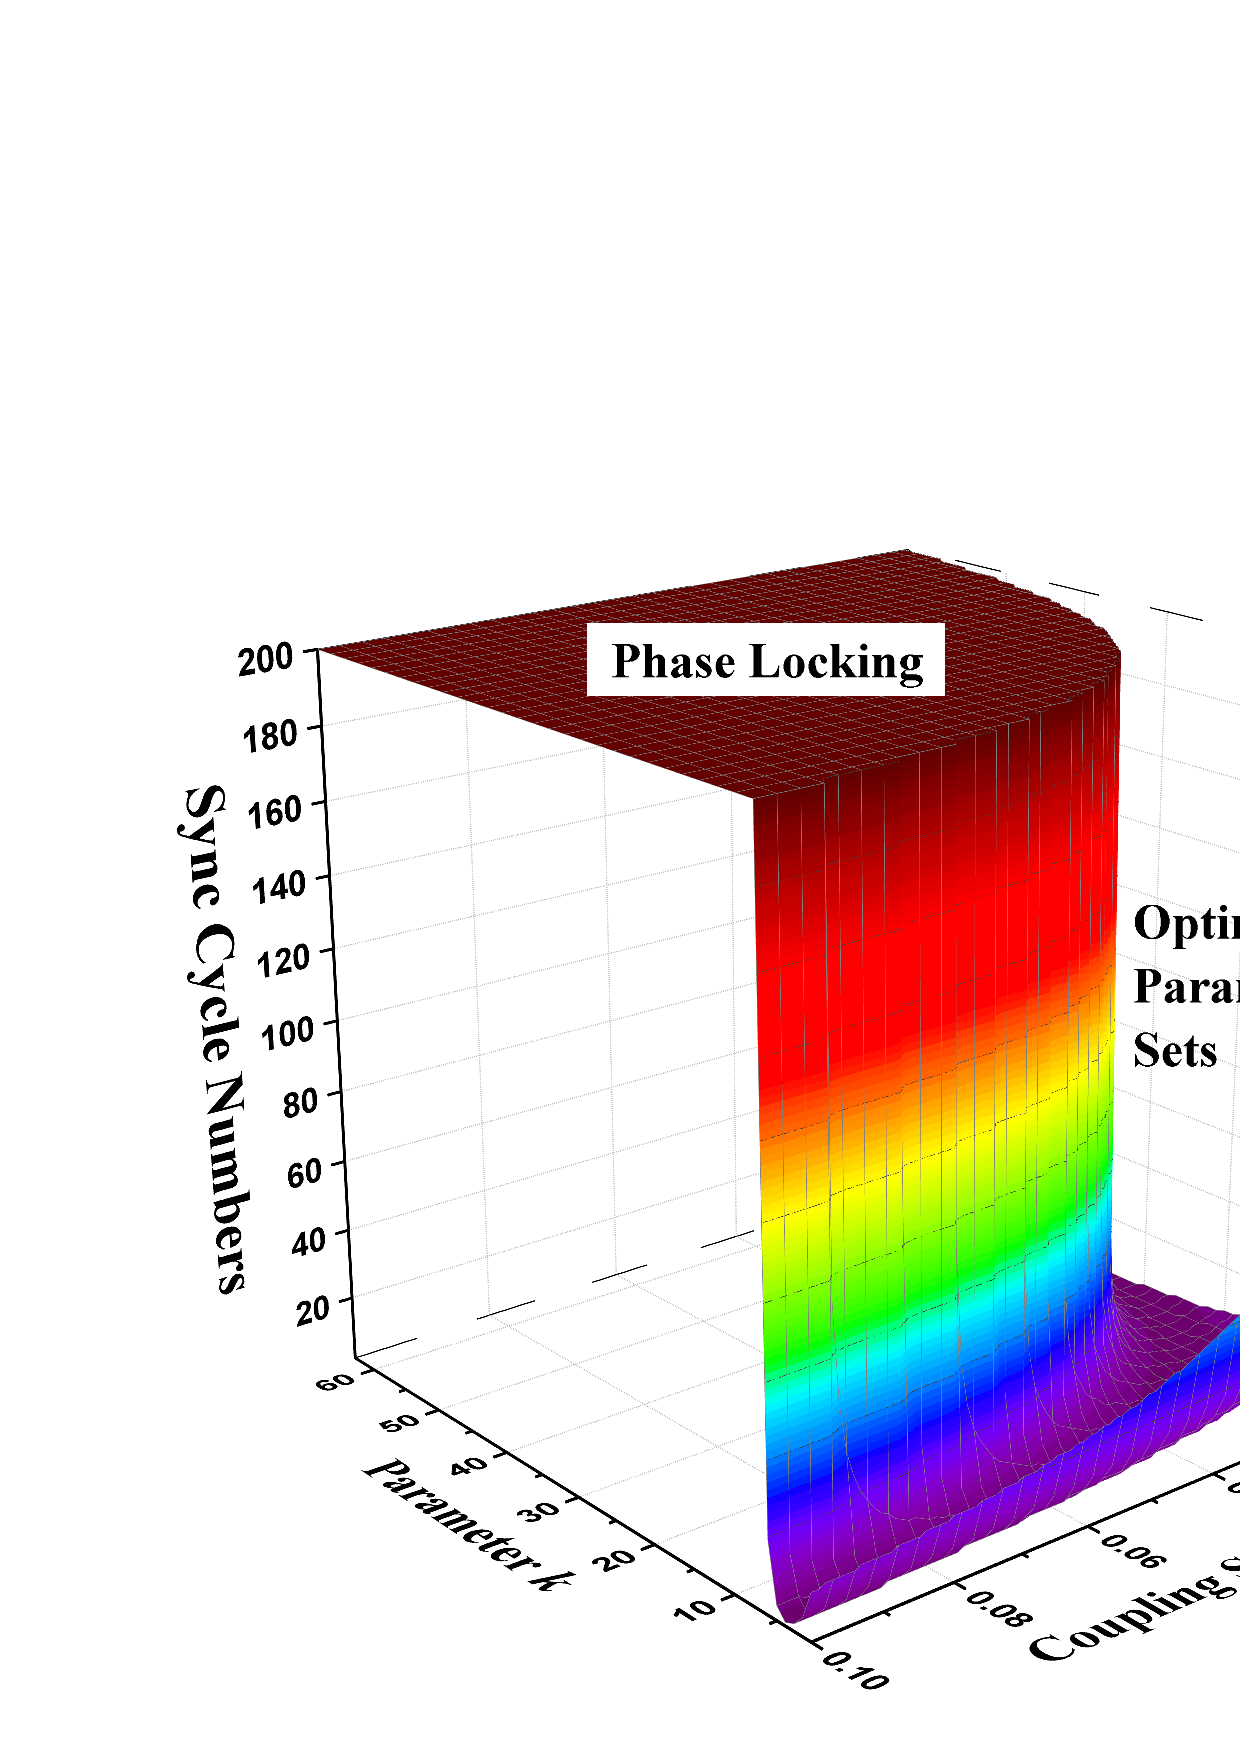
\includegraphics[width=3.5in]{Fig6_ParaK_Optimize}\\
  \caption{Various parameter $k$ under different coupling strength $\varepsilon$}
  \label{Fgi6_ParaK Optimize}
\end{figure}

\begin{figure}
  \centering
  % Requires \usepackage{graphicx}
  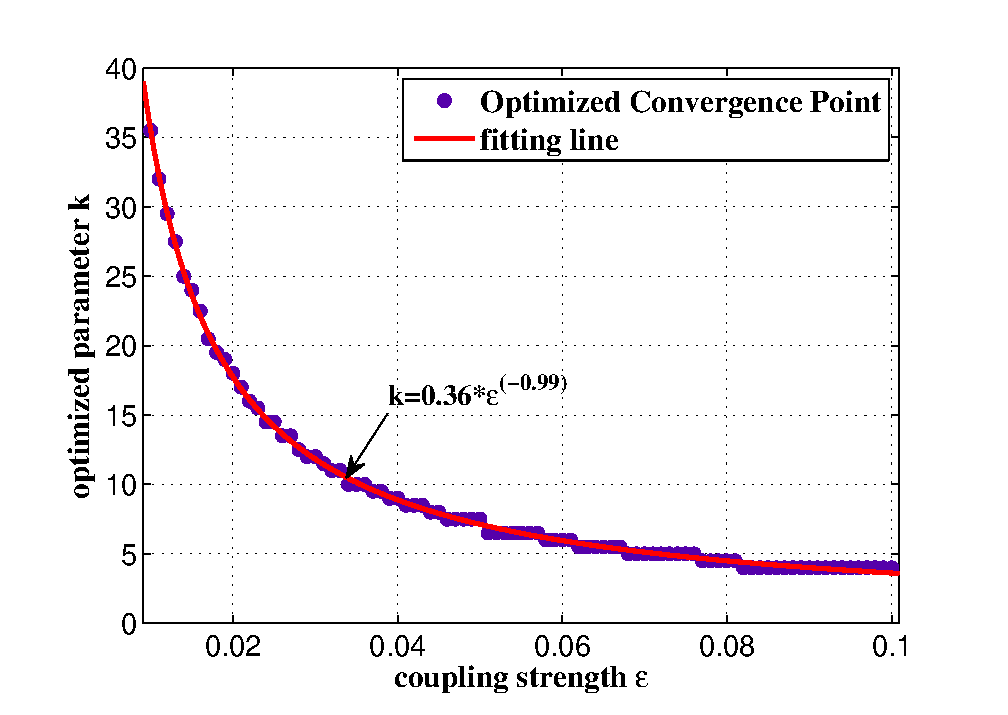
\includegraphics[width=3.5in]{Fig6_K_vs_e}\\
  \caption{Optimized parameter $k$ under different coupling strength $\varepsilon$}
  \label{Fgi6_K_vs_e_opt}
\end{figure}
\subsection{Time-efficient Optimization of PCO Model}
Under the sensing network described above, the novel Quadratic Polygon Model can be optimized according to (\ref{interaction between para k and coupling strength}). To modifies parameter $k$, synchronization process of the testing system needs to be carried out under various network coupling strength $\varepsilon$ and different Quadratic Polygon Models with different parameter $k$. In the test region, $\varepsilon$ raises from 0.01 to 0.10 with a step of 0.001 and $k$ naturally grows from 1 to 60, traversing every positive number. Numbers of cycles to reach synchronization are drawn in Fig.\ref{Fgi6_ParaK Optimize}. Despite the phase locking region, the optimal parameter sets correspond to the trough which indicates the minimum time collapse to reach synchronization. Select the parameters $k$ and $\varepsilon$ with the least synchronize cycles and employ the rational fitting model, relations of the optimized parameter sets are shown in Fig.\ref{Fgi6_K_vs_e_opt}. The fitting result claims that $k$ can be calculated by $k=0.36 \varepsilon^{-0.99}$. This result will be applied in the following contrast with traditional methods.

\subsection{Synchronous Sensing of PCO Models in Dynamic Sensing Networks}

\begin{figure}[!t]
\centering
\includegraphics[width=3.5in]{Fig8_RealTestBed.eps}
\caption{Dynamic interruptions on PCO synchronization performance}
\label{Fig_Exp_compare}
\end{figure}

Dynamic sensing network management implies sensing nodes dynamically leave and join the network, and the interruption brought to the network transient stability depends on the dynamic node scale. The time required to synchronize network under various dynamic node scale is presented in Fig. 7. 2 types of dynamic interrupts were introduced at t=50s and t=80s, former is 10 nodes joining in, latter is 5 nodes leaving. Apparently, the nodes leaving event do not interfere present synchronization state of the network, yet nodes joining will bring step change. 3 PCO models were adopted separately to synchronize the sensing network.

Results show that under non-ideal environment the synchronization accuracy varies according to different models. Quadratic Polygon model reached the lowest phase shift error of the 3 models. Phase shifts brought by the node joint took different time to regain synchronization. Quadratic Polygon model took 5s, Advanced Delay Tanh Model took 24s and Kuramoto Model took over 30s. This means that Quadratic Polygon model performs a better synchronization accuracy and speed, even under non-identical frequency and time delays.

Synchronization error will be introduced into electrical quality measurement as described in section III. The measurement error is influenced by changing rate of the measured characters and time disorder. Metering of power consumption and harmonics are presented to certificate the effects of synchronize accuracy on power quality measurement. Simulation data was measured in residential standard electrical environment 220V/50Hz, and the power quality characters�� measuring accuracy is important for information mining. The synchronization methods will bring various measuring error according to the time accuracy. Residential power characters�� data samples were collected and, to get a typical result, high-power electrical appliances were switched on and off to introduce interruptions. The power consumption fluctuates from 5kW to 10kW, with a step change every 50s. Based on (\ref{temporal_measure_error})the time synchronization��s influence on temporal measuring error is shown in table \ref{table_I}.

It can be figured out from the result that time synchronization accuracy has effect on temporal measuring error. Although the errors�� magnitude is not that large when compared with the measured data, yet in large scale analysis and data mining, the error is not ignorable. Since the Quadratic Polygon Model reaches the highest accuracy in Fig. \ref{Fig_Exp_compare}, it also brought in the least temporal error in the 3 models.
\subsection{Fault Localization with Synchronized Measurement}

To validate the synchronization in electrical fault diagnosis, voltage sag source localization is an appropriate test. System trajectory slope method \cite{voltage_sag_method} which is a widely authenticated way in voltage sag source location is employed in the simulation. The power quality parameters at the meter follows following principle:
\begin{equation}
\label{voltage_sag_local_method}
\begin{split}
|V\cos\theta_2| &= -RI + E_{1}\cos\theta_1(upstream) \\
|V\cos\theta_2| &= RI - E_{1}\cos\theta_1(downstream) \\
\end{split}
\end{equation}
$V,I$ stand for the voltage and current at the measuring point. $E_1$ stand for the supply voltage from upstream source. $R$ denotes the resistance between the measuring point and the upstream source. The direction of stream is determined by the current orientation. When a voltage sag occurs, the earth impendence at the measuring point changes and the voltage and current values varies accordingly. Nevertheless, based on (\ref{voltage_sag_local_method}), the values series of voltage and current will keep the positive or negative slope of $R$ which depends on the position of the metering node. Thus, it is able to locate whether the voltage sag source is in the upstream of downstream of this node. With numerous distributed metering nodes on the demand side, the voltage sag source can be located. Since the earth impendence $R$ changes overtime, the system slope of $V$ and $I$ does not strictly stay constant. Therefore, the time accuracy is crucial in detecting the voltage sag event. Low synchronization precision will lead to temporal offset in selecting measuring data, and influence the detection result.

The simulation sample of electrical network set is shown in Fig. \ref{Fig_Voltsag_Exp_set}. The Source supplies 3 phase 380$V$ after the transformer and 3 different types of loads are organized, which are composed of nonlinear resistance load, linear resistance load and an asynchronous motor. These 3 types of loads represent the most electrical appliances. A simulation is carried out within simulation environment Simulink.
\begin{figure}[!t]
\centering
\includegraphics[width=3.5in]{Fig9_VoltageSagExpSet}
\caption{Voltage sag source localization verification electrical model}
\label{Fig_Voltsag_Exp_set}
\end{figure}

Set 3 false sources at different time points, M1, M2, M3, as shown in Fig.\ref{Fig_Voltsag_Exp_set}. M1, M2, M3 are short-circuit fault, while M1 is set at bus line, and M2, M3 are set in local lines at user side.
With various synchronization models, each locate the voltage sag source 220 times, the locating result is shown in table \ref{table_II}.

From the result, it can be figured out that the 3 types of faults can be detected from the 3 different meters. However, for the sake of various synchronization accuracy, the localizing precision differs thoroughly.  Detection with Kuramoto model synchronization reaches the lowest precision of the 3 models while the new quadratic polygon model almost catches the fault every time. This experiment confirms that the amendment of the pulse coupled oscillator model, through increasing  synchronization accuracy of the measuring device, will reduce the fault localization error, and improve the whole safety of the cyber-physical energy system described in Section III.


\section{Conclusion}

Synchronous sensing is very important in power safety supervision in cyber-physical energy system. Synchronization method is required to be time-efficient, accurate and scalable in dynamic sensing networks. This paper proposed a new dynamic model for pulse-coupled oscillators synchronization method, to improve synchronization time efficiency and accuracy. By both theoretical and simulative analysis, models�� influence on PCO method performance is inquired and the coefficient of model parameters and coupling strength $\varepsilon$ is examined. In application of power network safety supervision on voltage sag localization under cyber-physical energy system, simulation experiments were carried out to evaluation PCO method. Result indicated that the new Quadratic Polygon Model fulfilled the time-efficiency and data measuring reliability requirements in dynamic sensing networks, and the fault localization exactitude was improved.
\begin{table}[!t]
\renewcommand{\arraystretch}{1.3}
\caption{TEMPORAL MEASURING ERROR FOR POWER QUALITY CHARACTERS (FIRST ELEMENT: AVERAGE ERR; SECOND ELEMENT: MAX ERR)}
\label{table_I}
\centering
\begin{tabular}{|c|c|p{7.6em}<{\centering}|p{7.6em}<{\centering}|}
\hline
\multirow{2}{*}{\textbf{Power Quality}} &
\multicolumn{3}{c|}{\textbf{PCO Model}} \\
\cline{2-4}
  & \textbf{Kuramoto Model} & \textbf{Advanced Delay Tanh Model} & \textbf{Quadratic Polygon Model} \\
\hline
Power/kW & (0.063, 1.521) & (6.2*e-4, 0.012) & (2.3*e-4, 0.003)  \\
\hline
3th Harmonic\footnotemark &	(0.182, 0.384) &	(1.8*e-3, 2.7*e-3)	& (7.0*e-4, 8.4*e-4) \\
\hline
5th Harmonic &	(0.073, 0.141) &	(7.2*e-4, 1.1*e-3)	& (2.7*e-4, 3.2*e-4) \\
\hline
7th Harmonic &	(0.027, 0.082) &	(2.7*e-4, 4.0*e-4)	& (1.0*e-4, 1.2*e-4) \\
\hline
\end{tabular}
\end{table}
\footnotetext{The harmonics are calculated with the power and voltage data. Voltage fluctuates slightly around 220$V$, and is not listed in the paper.}

\begin{table}[!t]
\renewcommand{\arraystretch}{1.3}
\caption{VOLTAGE SAG SOURCE LOCALIZATION ERROR}
\label{table_II}
\centering
\begin{tabular}{|c|c|p{7.5em}<{\centering}|p{7em}<{\centering}|}
\hline
\textbf{Fault Source} & \textbf{Kuramoto Model} & \textbf{Advanced Delay Tanh Model} & \textbf{Quadratic Polygon Model}  \\
\hline
M1 & 11.82\% & 2.73\% & 0.91\% \\
\hline
M2 & 5.45\% & 1.82\% & 0.45\% \\
\hline
M3 & 6.36\% & 1.82\% & 0.91\% \\
\hline
\end{tabular}

\end{table}

To further enhance the safety supervision in cyber physical energy system through raising synchronization accuracy, the non-identical frequencies and transmission delay of the sensing network should be considered in the design of pulse-coupled oscillators�� method. Specific theoretical analysis of discrete metering and synchronization process is to be carried out. Sensing network topology's impact on fault diagnosis also needs to be verified.

% Note that IEEE does not put floats in the very first column - or typically
% anywhere on the first page for that matter. Also, in-text middle ("here")
% positioning is not used. Most IEEE journals use top floats exclusively.
% Note that, LaTeX2e, unlike IEEE journals, places footnotes above bottom
% floats. This can be corrected via the \fnbelowfloat command of the
% stfloats package.



% if have a single appendix:
%\appendix[Proof of the Zonklar Equations]
% or
%\appendix  % for no appendix heading
% do not use \section anymore after \appendix, only \section*
% is possibly needed

% use appendices with more than one appendix
% then use \section to start each appendix
% you must declare a \section before using any
% \subsection or using \label (\appendices by itself
% starts a section numbered zero.)
%


%\appendices
%\section{Proof of the First Zonklar Equation}
%Appendix one text goes here.

% you can choose not to have a title for an appendix
% if you want by leaving the argument blank
%\section{}
%Appendix two text goes here.


% use section* for acknowledgement
%\section*{Acknowledgment}


%The authors would like to thank...


% Can use something like this to put references on a page
% by themselves when using endfloat and the captionsoff option.
\ifCLASSOPTIONcaptionsoff
  \newpage
\fi



% trigger a \newpage just before the given reference
% number - used to balance the columns on the last page
% adjust value as needed - may need to be readjusted if
% the document is modified later
%\IEEEtriggeratref{21}
% The "triggered" command can be changed if desired:
%\IEEEtriggercmd{\enlargethispage{-5in}}

% references section

% can use a bibliography generated by BibTeX as a .bbl file
% BibTeX documentation can be easily obtained at:
% http://www.ctan.org/tex-archive/biblio/bibtex/contrib/doc/
% The IEEEtran BibTeX style support page is at:
% http://www.michaelshell.org/tex/ieeetran/bibtex/
\bibliographystyle{IEEEtran}
% argument is your BibTeX string definitions and bibliography database(s)
%\bibliography{IEEEabrv,../bib/PCO.bib}
%
% <OR> manually copy in the resultant .bbl file
% set second argument of \begin to the number of references
% (used to reserve space for the reference number labels box)
\begin{thebibliography}{30}

\bibitem{CPS_In_SmartGrid}
S. Karnouskos, "Cyber-physical systems in the smart grid," \emph{in IEEE Conf. 9th Industrial Informatics (INDIN)}, 2011, 20-23.

\bibitem{CPES_Intro}
C.A. Macana, N. Quijano, E. Mojica-Nava, "A survey on cyber physical energy systems and their applications on smart grids", in \emph{Innovative Smart Grid Technologies (ISGT Latin Ame}.2011, pp. 1-7.

\bibitem{CSP}
X. Wang, S. Wang, "Collaborative signal processing for target tracking in distributed wireless sensor networks," \emph{J. Parallel and Distrib. Comput.}, vol.67, no.5, pp. 501-515, Feb. 2007.

\bibitem{Fault_Analysis_Intro}
T. Brennan, "Market failures in real-time metering," \emph{Journal Regulatory Economics}, vol.26, no.2, pp.119-139, Sept. 2004.

\bibitem{SyncMethodInWSN}
Y. C. Wu, Q. Chaudhari, and E. Serpedin, "Clock synchronization of wireless sensor networks, " \emph{IEEE Signal Process. Mag.}, vol.28, no.1, pp.124-138, Jan. 2011.

\bibitem{TPSN}
S. Ganeriwal, R Kumar, M B. Srivastava. "Timing-sync protocol for sensor networks," \emph{ACM Proceedings of the 1st international conference on. Los Angeles, California, USA}, 2003: 138-149.

\bibitem{RBS}
J. Elson, L. Girod, and D. Estrin, "Fine-grained network time synchronization using reference boradcasts, " \emph{ACM SIGOPS Oper. Syst. Rev.}, vol.36, no.SI, p.147, Dec. 2002.

\bibitem{FTSP}
M Mar��ti, B Kusy, G Simon, et al. "The flooding time synchronization protocol," \emph{in Proceedings of the 2nd international conference on Embedded networked sensor systems-SenSys}, 2004, pp.39-49.

\bibitem{Glossy}
F. Ferrari, M. Zimmerling, L. Thiele, et al. "Efficient network flooding and time synchronization with glossy," \emph{Information Processing in Sensor Networks (IPSN), 2011 10th International Conference on}, pp.73-84, 2011.

\bibitem{PCO_Scaglione_2005}
Yao-win H., A. Scaglione. "A scalable synchronization protocol for large scale sensor networks and its applications," \emph{IEEE J. Sel. Areas in Commun.} vol.23 no.5, pp.1085-1099, May, 2005.

\bibitem{PCO_Scaglione_2011}
R. Pagliari, A. Scaglione, "Scalable network synchronization with pulse-coupled oscillators," \emph{IEEE Trans. on, Mobile Comput.} vol.10, no.3, pp.392-405, Mar., 2011.

\bibitem{PCO_Doyle_PRF_2012}
Y.Q. Wang, F.J. Doyle, "Optimal phase response functions for fast pulse-coupled synchronization in wireless sensor networks," \emph{IEEE Trans. on, Signal Process.}, vol.60, no.10, pp.5583-5588, Oct., 2012.

\bibitem{PCO_Doyle_PRF_2013}
Y.Q. Wang, F. Nunez, F.J. Doyle. "Increasing sync rate of pulse-coupled oscillators via phase response function design: theory and application to wireless networks," \emph{IEEE Trans. on, Control Systems Technology}, vol.21, no.4, pp.1455-1462, Jul, 2013.

\bibitem{PCO_Doyle_Stat_Anly_2013}
Y.Q. Wang, F. Nunez, F.J. Doyle. "Statistical analysis of the pulse-coupled synchronization strategy for wireless sensor networks," \emph{IEEE Trans. on, Signal Process.}, vol.61, no.21, pp.5193-5204, Nov., 2013.

\bibitem{PCO_CAS_2011}
Z. L. An, H. S. Zhu, X. R. Li, et al. "Nonidentical linear pulse-coupled oscillators model with application to time synchronization in wireless sensor networks. "\emph{IEEE Trans. on Ind. Electron.}, vol.58, no.6, pp.2205-2215, Jun., 2011.

\bibitem{Neuroscience_2007}
E. M. Izhikevich, \emph{Dynamical systems in neuroscience: the geometry of excitability and bursting,} MIT Press, 2007.

\bibitem{NewFrontierOfSG}
X. Yu, C. Cecati, T. Dillon and M. Simoes. "The new frontier of smart grids," \emph{IEEE Trans. Ind Electron.}, vol.5, no.3, pp.49-63, Sept. 2011.

\bibitem{Fault_Local_impendence_based1}
A. A. Girgis, C. M. Fallon, and D. L. Lubkeman, "A fault location technique for rural distribution feeders, "\emph{IEEE Trans. Ind. Appl.}, vol.29, no. 6, pp.1170-1175, Dec. 1993.

\bibitem{Fault_Local_impendence_based2}
M.S. Choi, S.J. Lee, D. S. Lee, and B. G. Jin, "A new fault location algorithm using direct circuit analysis for distribution systems, "\emph{IEEE Trans. Power Del.}, vol.19, no.1, pp.25-41, Jan. 2004.

\bibitem{Fault_Local_freq_based}
A. Borghetti, M. Bosetti, M.D. Sivestro, C. A. Nucci, and M. Paolone, "Continuous-wavelet transform for fault location in distribution power networks: Definition of mother wavelets inferred from fault originated transients,"\emph{IEEE Trans. Power Syst,}, vol.23, no.2, pp.380-388, May, 2008.

\bibitem{Fault_Local_Sparse}
R.A.Pereira, L.G.Silva, M.Kezunovic, and J.R. Mantovani, "Inproved fault location on distribution feeders based on matching during-fault voltage sags," \emph{IEEE Trans. Power Del.}, vol.24, no.2, pp.852-862, Apr. 2009.

\bibitem{IEC61588}
"IEEE Standard for a precision clock synchronization protocol for networked measurement and control systems ", pp.C1-274, 2009.

\bibitem{GPS_sync}
H. Ukai, K. Nakamura, and N. Matsui, "DSP- and GPS-based synchronized measurement system of harmonics in wide-area distribution system, "\emph{IEEE Trans. Ind. Electron.}, vol.50, no.6, pp.1159-1164, Dec. 2003.

\bibitem{Voltage_sag_local_Texas}
Y. Dong, C. Zheng and M. Kezunovic, "Enhancing accuracy while reducing comutation complexity for voltage-sag-based distribution fault location",\emph{IEEE Trans. on, Power Deliv.}, vol.28, no.2, pp.1202-1212, 2013.

\bibitem{Fault_Local_Using_Current}
S. Das, N. Karnik, and S. Santoso, "Distribution fault-locating algorithms using current only," \emph{IEEE Trans. Power Del.}, vol.27, no.3, pp.1144-1153, Jul, 2012.

\bibitem{Fault_Local_Using_Voltage}
Z. Galijasevic and A. Abur, "Fault localization using voltage measurements", \emph{IEEE Trans. on, Power Deliv.} vol.17, no.2, pp.441-445, 2002.

\bibitem{WSN_In_SmartGrid}
V. Gungor, B. Lu, G. Hancke, "Opportunities and challenges of wireless sensor networks in smart grid," \emph{IEEE Trans. Ind Electron.}, vol.57, no.10, pp.3557-3564, 2010.

\bibitem{Sync_Intro_InWSN_Book}
E. Serpedin, Q. Chaudhari, "Synchronization in wireless sensor Nnetworks: parameter estimation, performance benchmarks and protocols", \emph{Cambridge University Press},2009, Aug. 31.

\bibitem{PCO_Theory_1990}
R.E. Mirollo, S.H. Strogatz. "Synchronization of pulse-coupled biological oscillators,"  \emph{SIAM J. Appl. Math.}, vol.50, no.6, pp.1645-1662, Dec., 1990.

\bibitem{PCO_in_SG}
F. Dorfler, M. Chertkov, and F. Bullo, "Synchronization in comlex oscillator networks and smart grids, "\emph{Proc. Natl. Acad. Sci. USA}, vol.110, no.6, pp.2005-2010, Feb. 2013.

\bibitem{AMI}
N. Liu, J. Chen, L. Zhu, J. Zhang, and Y. He, "A Key Management Scheme for Secure Communications of Advanced Metering Infrastructure in Smart Grid, "\emph{IEEE Trans. Ind. Electron,} vol.60, no.10, pp.4746-4756, Oct. 2013.

\bibitem{fault_diagnosis_use_WSN}
R. C. Luo and O. Chen, "Mobile Snesor Node Deployment and Asynchronous Power Management for wireless sensor networks, "\emph{IEEE Trans. Ind. Electron.,} vol.59, no.5, pp.2377-2385, May 2012.

\bibitem{PowerReliabilityTheory}
R. C. Leou, C. N. Lu. "Adjustment of the extemal network��s measurements and its effect on the power mismatch analysis", \emph{Proeeedings of IEEE Industry Application Society Annual Meeting}, Vol.3, pp.2072-2076, 1999.

\bibitem{Kuramoto}
Kuramoto, Yoshiki, \emph{Chemical Oscillations, Waves, and Turbulence}, Springer-Verlag, New York, 1984, pp. 164.

\bibitem{PCO_Neuroscience_Theory_1997}
F.C. Hoppensteadt and E.M. Izhikevich, \emph{Weakly Connected Neural Networks}, Springer, 1997.

\bibitem{nonlinear_system}
H. K. Khalil, \emph{Nonlinear Systems}, Englewood Cliffs, NJ: Prentice-Hall, 2002, pp.1-42.

\bibitem{Hodgkin-Huxley}
B. Ermentrout, "Type I membrances, phase resetting curves, and synchrony", \emph{Neural Comput.}, vol.8, no.5, pp. 979-1001, Apr. 1996

\bibitem{DLT_645_2007}
DL/T 645-2007, "Multi-function Watt-hour Meter Communication Protocol", 2007

\bibitem{voltage_sag_method}
C. Li, T. Tayjasanant, W. Xu, et al. ��Method for voltage-sag-source detection by investigating slope of the system trajectory��. \emph{in IEE Proc, Gener. Transm. Distrib., }vol.150, no.3, pp.367-372, Mar. 2003.

%\bibitem{Time_Sync_Intro}
%D. Ingram, P. Schaub, D. Campbell, and R. Taylor "Evaluation of precision time synchronisation methods for substation applications" \emph{IEEE Symposium on Precision Clock Synchronization for Measurement, Control and Communication}, 2012:1-6

%\bibitem{Voltage_sag_sync}
%Y. Sillapawicharn and Y. Kumsuwan, "An improvement of synchronously rotating reference frame based voltage sag detection for voltage sag compensation applications under distorted grid voltages", \emph{IEEE PEDS}, 2011.

%\bibitem{Voltage_sag_intro}
%M. F. McGranaghan, D. R. Mueller, and M.J. Samotyj,. ��Voltage sags in industrial systems��. \emph{IEEE Trans. on Ind. Appl.}, vol.29, no.2, pp.397-403, Feb., 1993.

\end{thebibliography}
% biography section
%
% If you have an EPS/PDF photo (graphicx package needed) extra braces are
% needed around the contents of the optional argument to biography to prevent
% the LaTeX parser from getting confused when it sees the complicated
% \includegraphics command within an optional argument. (You could create
% your own custom macro containing the \includegraphics command to make things
% simpler here.)
%\begin{IEEEbiography}[{\includegraphics[bb = 0 0 96 132, width=1in,height=1.25in,clip,keepaspectratio]{XUE_WANG}}]{Xue Wang}
% or if you just want to reserve a space for a photo:
%\newpage
%\begin{spacing}{1.0}
\begin{IEEEbiography}[{\includegraphics[width=1in,height=1.25in,clip,keepaspectratio]{YoudaLiu}}]{Youda Liu}
(S'14)received the B.S. degree in mechanical engineering in 2011 from Tsinghua University, Beijing, China,where he is currently working toward the Ph.D. degree with the Department of Precision Instrument.

His research interests include signal and information processing, wireless sensor networks and Cyber-physical systems.
\end{IEEEbiography}
%\end{spacing}
\begin{IEEEbiography}[{\includegraphics[width=1in,height=1.25in,clip,keepaspectratio]{XUE_WANG_G}}]{Xue Wang}
%Biography text here.
(M'08)received the M.S.degree in
measurement and instrument from Harbin Institute of Technology, Harbin, China, in 1991 and the Ph.D. degree in mechanical engineering from Huazhong University of Science and Technology, Wuhan, China, in 1994.

From 1994 to 1996, he was a Postdoctoral Fellow in electrical power systems with Huazhong University of Science and Technology. He then joined the Department of Precision Instrument, Tsinghua University, Beijing, China, where he is currently a Professor and Vice Dean of Department of Precision Instrument , Tsinghua University. From May 2001 to July 2002, he was a Visiting Professor with the Department of Mechanical Engineering, University of Wisconsin, Madison. His research interests include engineering measurement, advanced metering infrastructure, wireless sensor networks, Cyber-physical systems, and intelligent maintenance.

Dr. Wang is a member of the IEEE Instrumentation and Measurement Society, Computer Society, Computational Intelligence Society, and Communications Society. He received
\end{IEEEbiography}
% insert where needed to balance the two columns on the last page with
% biographies
%\newpage
%\begin{spacing}{1.0}
\begin{IEEEbiography}[{\includegraphics[width=1in,height=1.25in,clip,keepaspectratio]{XINYAO_SUN}}]{Xinyao Sun}
received the B.S. degree in mechanical engineering in 2007 from Tsinghua University, Beijing, China,where he is currently working toward the Ph.D. degree with the Department of Precision Instrument.

His research interests include signal and information processing, wireless sensor networks, and Cyber-physical systems.
\end{IEEEbiography}
%\end{spacing}
\begin{IEEEbiography}[{\includegraphics[width=1in,height=1.25in,clip,keepaspectratio]{JIANGWEI_WU}}]{Jiangwei Wu}
received the B.S. degree in measurement and instrument in 2007 and M.S. degree in instrument science and technology in 2010 from Harbin Institute of Technology, HarBin, China. He is currently working toward the Ph.D. degree with the Department of Precision Instrument in Tsinghua University, Beijing, China.

His research interests are in the area of the power quality monitoring in wireless sensor networks and Cyber-physical systems.
\end{IEEEbiography}
% You can push biographies down or up by placing
% a \vfill before or after them. The appropriate
% use of \vfill depends on what kind of text is
% on the last page and whether or not the columns
% are being equalized.

% Can be used to pull up biographies so that the bottom of the last one
% is flush with the other column.
%\enlargethispage{-5in}



% that's all folks
\end{document}


